\documentclass[11pt]{article}

\usepackage[utf8]{inputenc}
\usepackage[T1]{fontenc}
\usepackage{lmodern}
\usepackage[margin=1in]{geometry}
\usepackage{amsmath,amssymb}
\usepackage[version=4]{mhchem}
\usepackage{graphicx}
\usepackage{booktabs}
\usepackage{siunitx}
\usepackage{natbib}
\usepackage{authblk}
\usepackage{caption}
\usepackage{xurl}
\usepackage[hidelinks]{hyperref}

\graphicspath{{figures/}}
\setcitestyle{authoryear,round}
\captionsetup{font=small,labelfont=bf}
\sisetup{detect-all,group-separator={,}}
\DeclareSIUnit\year{yr}

\title{\textbf{Globally consistent Land Environmental Assessment Factors (LEAFs)
for soil organic carbon, soil erosion, and terrestrial acidification
in support of SBTN Land v2 Targets}}

\author[1]{Cristóbal Loyola}
\affil[1]{World Wildlife Fund (WWF), Washington, DC, USA \\ \texttt{cristobal.loyola@wwfus.org}}

\date{\today}

\begin{document}

\maketitle

\begin{abstract}
\noindent
Setting credible, science-based land targets requires companies to compare the
environmental performance of their sourcing landscapes against ecoregion-specific
reference conditions, yet site-level primary data are rarely available across global
supply chains. We present \emph{Land Environmental Assessment Factors} (LEAFs): a
global, openly licensed dataset of default factors for three soil-quality indicators
---soil organic carbon (SOC), soil erosion, and terrestrial acidification---together
with a reproducible Python pipeline (\texttt{sbtn\_leaf}) that generates them. SOC
factors are produced by running the Rothamsted Carbon (RothC) model forward to 2030
on a harmonized stack of SoilGrids, satellite climate, and crop-specific yield and
residue inputs; soil-erosion factors apply the Revised Universal Soil Loss Equation
(RUSLE) to Global Soil Erosion Modelling (GloSEM) base layers with crop and
management cover-factors; and terrestrial-acidification factors are derived from
published fate and sensitivity factors normalized to \ce{SO2}-equivalents. Factors are
resolved for 42 land-use classes under up to eight management combinations (irrigation,
tillage, and residue management) and are delivered as native-resolution rasters and as
area-weighted summaries for terrestrial ecoregions, countries, and subcountry units.
Across ecoregions the 2030 SOC factors average \SI{34.7}{\tonne\,C\per\hectare},
baseline soil-erosion rates average \SI{48.8}{\tonne\per\hectare\per\year} (median
\SI{15.3}{}), and acidification factors span more than an order of magnitude between
biogeographic realms. Adopting reduced tillage raises projected SOC by on the order of
\SI{1.6}{\tonne\,C\per\hectare} (\(\approx\)5\%) for a representative cereal. All code,
documentation, and factor tables are released under a CC0 license so that organizations
can apply the factors directly or regenerate customized factors from primary data.
\end{abstract}

\section{Introduction}
\label{sec:intro}

Land use is among the largest drivers of biodiversity loss, soil degradation, and
greenhouse-gas emissions, and it is increasingly central to corporate sustainability
commitments. The Science Based Targets Network (SBTN) Land methodology asks companies
to set targets that move their sourcing landscapes toward a ``safe operating space''
consistent with planetary boundaries \citep{rockstrom2009,sbtnland2025}. Operationally,
this requires two ingredients: an ecoregion-specific \emph{threshold} that defines safe
conditions for a given soil-quality indicator, and an \emph{assessment factor} that
estimates the indicator value associated with a company's actual land use and
management. While thresholds are derived from reference ecosystems, the assessment
factor must be estimated for every combination of commodity, geography, and management
practice a company may operate---a quantity that is almost never measured directly at
scale.

Life-cycle assessment (LCA) provides regionalized characterization factors for related
impacts, but these are typically tuned to product-level accounting rather than to the
ecoregional, practice-sensitive comparisons that target-setting demands. There is
therefore a need for \emph{default} factors that are (i) globally complete, (ii)
spatially explicit at ecoregional granularity, (iii) responsive to land-management
choices, and (iv) transparent and reproducible so that organizations with primary data
can refine them.

This paper introduces Land Environmental Assessment Factors (LEAFs) to meet that need.
We build on the global SOC modelling framework of \citet{morais2019} and
\citet{teixeira2021}, extend it to soil erosion and terrestrial acidification, and
package the entire workflow as an open-source Python library. Our contributions are: (1)
a harmonized, global, ecoregion-resolved dataset of default factors for three
soil-quality indicators under multiple management scenarios; (2) a reproducible,
tested software implementation (\texttt{sbtn\_leaf}) covering data harmonization,
biogeochemical and empirical modelling, spatial aggregation, and export; and (3) an
analysis of the resulting global patterns and of the sensitivity of SOC factors to
conservation practices. The factors are designed to plug directly into the SBTN Land
accounting framework \citep{sbtnagile2025}.

\section{Materials and Methods}
\label{sec:methods}

\subsection{Spatial framework and overview}
All factors are computed on a common spatial framework built from the Unique Homogeneous
Thermal--Humidity (UHTH) zonation of \citet{morais2019}, which partitions the globe
following the FAO Global Agro-Ecological Zones (GAEZ) suitability framework
\citep{gaez2012}. Every input layer is harmonized---reprojected and resampled---to this
common grid before calculation. After per-pixel factors are produced, they are
aggregated by area-weighted zonal statistics to three reporting units: terrestrial
ecoregions \citep{olson2001}, countries, and subcountry administrative units. Reporting
at ecoregion level is the default because it best matches the resolution of SBTN
thresholds; country averages are retained only as a last resort because of their low
spatial representativeness. The overall workflow comprises four stages---data gathering
and processing, harmonization, factor calculation, and zonal aggregation---applied
consistently to each indicator.

\subsection{Input datasets}
Table~\ref{tab:inputs} summarizes the primary inputs. Climate drivers are multi-year
means to represent typical rather than single-year conditions: monthly precipitation
from NASA GPM IMERG averaged over 2013--2023 \citep{huffman2020}, and monthly
temperature from the GLDAS Catchment Land Surface Model \citep{rodell2004}. Soil
properties (organic-carbon stock for 0--30~cm, and clay and sand fractions for
15--30~cm) are taken from SoilGrids \citep{poggio2021}. Yields combine FAOSTAT national
statistics \citep{faostat} with the spatially disaggregated SPAM~2020 product
\citep{spam2020}. Soil-erosion base layers come from the GloSEM platform
\citep{borrelli2017,borrelli2022,panagos2015}, and acidification fate--sensitivity
factors from \citet{roy2014}.

\begin{table}[t]
\centering
\caption{Primary input datasets used to generate the LEAFs.}
\label{tab:inputs}
\small
\begin{tabular}{@{}lll@{}}
\toprule
Variable & Source & Native resolution / notes \\
\midrule
Monthly precipitation & NASA GPM\_3IMERGM \citep{huffman2020} & \SI{0.1}{\degree}, 2013--2023 mean \\
Monthly temperature & GLDAS CLSM10 M v2.1 \citep{rodell2004} & \SI{1.0}{\degree} \\
SOC stock (0--30 cm) & SoilGrids \citep{poggio2021} & \\
Clay fraction (15--30 cm) & SoilGrids \citep{poggio2021} & \\
Sand fraction (15--30 cm) & SoilGrids \citep{poggio2021} & reduced-tillage only \\
$R\cdot K_{st}\cdot LS$ base & GloSEM v1.1/1.3 \citep{borrelli2017} & \SI{25}{\km} \\
Crop yields & FAOSTAT \citep{faostat} + SPAM 2020 \citep{spam2020} & rainfed/irrigated splits \\
Residue parameters & IPCC \citep{ipcc2006,ipcc2019} & Table~\ref{tab:residues} \\
Acidification FF$\times$SF & \citet{roy2014} & \SI{2}{\degree}$\times$\SI{2.5}{\degree} \\
Land-use / UHTH zones & \citet{morais2019} & FAO GAEZ v2 \\
\bottomrule
\end{tabular}
\end{table}

\subsection{Soil organic carbon factors}
\label{sec:soc}

\paragraph{RothC model.} SOC factors are produced with the Rothamsted Carbon (RothC)
model \citep{coleman2024}, which simulates the turnover of organic carbon in
non-waterlogged topsoils, accounting for soil type, temperature, moisture, and plant
cover. RothC partitions soil carbon into five pools: decomposable plant material (DPM),
resistant plant material (RPM), microbial biomass (BIO), humified organic matter (HUM),
and inert organic matter (IOM). The active pools decompose with first-order kinetics
whose monthly rate is modulated by three dimensionless rate-modifying factors. The
temperature factor is
\begin{equation}
a = \frac{47.91}{1 + \exp\!\left(\dfrac{106.06}{T + 18.27}\right)},
\label{eq:rmf-temp}
\end{equation}
where $T$ is mean monthly air temperature (\si{\degreeCelsius}); a moisture factor $b$
is derived from the accumulated topsoil moisture deficit, which depends on rainfall,
evapotranspiration, and a clay-dependent maximum deficit; and a plant-cover factor $c$
takes the value $1.0$ for bare soil and $0.6$ when the soil is vegetated. A modified
tillage rate-modifying factor, adapted from \citet{hyun2024} using soil sand content and
SOC, is applied to represent conservation (reduced) tillage. Carbon enters the system as
monthly plant-residue inputs (and, optionally, farmyard manure), partitioned between DPM
and RPM by a ratio of 1.44 for agricultural crops and improved grassland, 0.67 for
unimproved grassland and scrub, and 0.25 for woodland \citep{coleman2024}. The model is
initialized from the SoilGrids SOC baseline and clay content and integrated forward
month by month; the SOC stock in the final projection year (2030 for the published
factors) is the SOC LEAF, expressed in \si{\tonne\,C\per\hectare}.

\paragraph{Potential evapotranspiration.} Because routine open-pan evaporation
measurements are unavailable globally, RothC's moisture deficit is driven by potential
evapotranspiration (PET) estimated with the Thornthwaite equation
\citep{thornthwaite1948}. For months with $T>0\,\si{\degreeCelsius}$,
\begin{equation}
\mathrm{PET} = 1.6 \cdot \frac{L}{12} \cdot \frac{N}{30}
\cdot \left(\frac{10T}{I}\right)^{a_\mathrm{T}},
\label{eq:pet}
\end{equation}
where $L$ is mean daily daylight hours, $N$ the number of days in the month, $I$ the
annual heat index $I = \sum_i (T_i/5)^{1.514}$ over months with $T_i>0$, and
$a_\mathrm{T} = 6.75\times10^{-7}I^3 - 7.71\times10^{-5}I^2 + 1.792\times10^{-2}I +
0.49239$. Daylight duration $L$ is obtained from the solar hour angle
$\omega_0$, with $\cos\omega_0 = -\tan\phi\,\tan\delta$, latitude $\phi$, and solar
declination $\delta = 23.44^{\circ}\sin\!\big(\tfrac{360^{\circ}}{365}(n-81)\big)$
evaluated at the middle day $n$ of each month. The location-based PET is converted to a
crop-specific value by multiplying by a monthly crop coefficient $K_c$, built from the
FAO-56 single-coefficient method \citep{allen1998} using stage values
$K_{c,\text{ini}}$, $K_{c,\text{mid}}$, and $K_{c,\text{late}}$ defined per crop and
thermal zone \citep{morais2019,chapagain2004}. Figure~\ref{fig:kc} illustrates a
representative $K_c$ curve.

\begin{figure}[t]
\centering
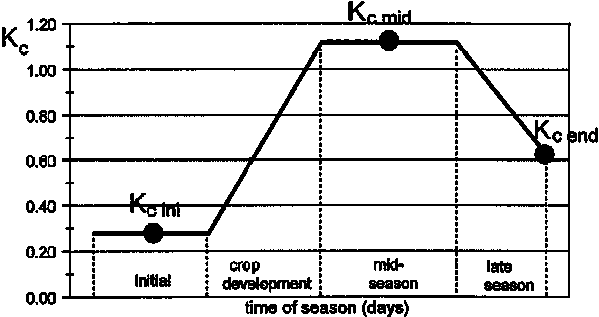
\includegraphics[width=0.62\textwidth]{K_Curve_example.png}
\caption{Example monthly crop-coefficient ($K_c$) curve constructed from FAO-56 stage
values and stage durations \citep{allen1998}, used to convert location-based potential
evapotranspiration into crop evapotranspiration.}
\label{fig:kc}
\end{figure}

\paragraph{Yields and residue inputs.} Plant-residue carbon inputs are derived from
commodity yields. To assign a yield to every UHTH zone where a crop can grow, a
hierarchical procedure is applied (implemented in
\texttt{create\_crop\_yield\_raster\_withIrrigationPracticeScaling}): (1) national
FAOSTAT yields and a calibration ratio to 2020 are computed; (2) SPAM 2020 rainfed,
irrigated, and total yields are averaged and rescaled by the FAOSTAT ratio; (3) where
SPAM data exist they are assigned, otherwise the FAOSTAT national value adjusted for
irrigation practice is used; (4) remaining gaps are filled by ecoregion and then biome
means; and (5) any residual gaps are filled by nearest-neighbour assignment. Yields are
converted to dry matter and then to above- and below-ground residue carbon following the
IPCC method \citep{ipcc2006,ipcc2019}:
\begin{align}
\mathrm{AG}(T) &= \mathrm{Crop}(T)\cdot \mathrm{Slope}(T) + \mathrm{Intercept}(T), \\
\mathrm{BG}(T) &= \big[\mathrm{Crop}(T) + \mathrm{AG}(T)\big]\cdot \mathrm{RS}(T),
\end{align}
where $\mathrm{Crop}(T)=\mathrm{Yield}(T)\cdot\mathrm{DRY}(T)$, and the slope,
intercept, dry-matter, and root-to-shoot ($\mathrm{RS}$) parameters are given in
Table~\ref{tab:residues}. A 50\% carbon content is assumed, and the resulting residue
is distributed across months following \citet{morais2019}.

\begin{table}[t]
\centering
\caption{IPCC residue parameters used to convert yields into above- and below-ground
residue carbon inputs \citep{ipcc2006,ipcc2019}.}
\label{tab:residues}
\small
\begin{tabular}{@{}lcccc@{}}
\toprule
Crop & Dry & Slope & Intercept & RS \\
\midrule
Barley & 0.89 & 0.98 & 0.59 & 0.22 \\
Seed cotton (unginned) & 0.85 & 1.07 & 0.85 & 0.19 \\
Maize & 0.87 & 1.03 & 0.61 & 0.22 \\
Rape / colza seed & 0.85 & 1.13 & 0.85 & 0.19 \\
Sorghum & 0.89 & 0.88 & 1.33 & 0.22 \\
Soya bean & 0.91 & 0.93 & 1.35 & 0.19 \\
Sunflower seed & 0.85 & 1.13 & 0.85 & 0.19 \\
Wheat & 0.89 & 1.51 & 0.52 & 0.23 \\
\bottomrule
\end{tabular}
\end{table}

\subsection{Soil-erosion factors}
\label{sec:erosion}
Soil-erosion factors estimate the annual rate of soil loss
(\si{\tonne\per\hectare\per\year}) using the Revised Universal Soil Loss Equation
(RUSLE):
\begin{equation}
RE = R\cdot K_{st}\cdot LS\cdot C\cdot P,
\label{eq:rusle}
\end{equation}
where $R$ is rainfall erosivity, $K_{st}$ soil erodibility corrected for the skeletal
fraction, $LS$ the slope-length and steepness factor, $C$ the cover-management factor,
and $P$ the support-practice factor. Because $R$, $K_{st}$, and $LS$ are independent of
land use, a single $R\cdot K_{st}\cdot LS$ base raster is precomputed from the
GloSEM layers \citep{borrelli2017,panagos2015} and reused for every commodity. Following
common practice in LCA characterization, $P$ is set to~1. The cover-management factor is
disaggregated into a crop component and a management component,
\begin{equation}
C_{\text{arable}} = C_{\text{crop}}\times C_{\text{mgmt}}, \qquad
C_{\text{mgmt}} = C_{\text{till}}\times C_{\text{res}}\times C_{\text{cover}},
\end{equation}
where crop $C$ values are assigned per commodity from \citet{borrelli2017},
$C_{\text{till}} \in \{1,\,0.35,\,0.25\}$ for conventional, reduced, and no-till
practices respectively, $C_{\text{res}} = 1 - 0.12\,F_{\text{res}}$ for the fraction of
land leaving residues, and $C_{\text{cover}} = 1 - 0.2\,F_{\text{cover}}$ for the
fraction using cover crops \citep{panagos2015}. The baseline factor assumes no
erosion-reducing practices; other scenarios are obtained by multiplying the baseline by
the corresponding $C_{\text{mgmt}}$.

\subsection{Terrestrial-acidification factors}
\label{sec:acid}
Terrestrial-acidification factors are obtained directly from the fate ($FF$) and soil
sensitivity ($SF$) factors of \citet{roy2014}, supplied on a
\SI{2}{\degree}$\times$\SI{2.5}{\degree} grid as the product $FF\times SF$ (in
\si{\mol} \ce{H+}\,\si{\per\litre}\,\si{\square\metre}\,\si{\per\kilogram}\,\si{\year}),
with corrections to the original calculations consistent with IMPACT World+ v2.0
\citep{impactworldplus}. No process modelling is performed; the published values are
renormalized to \ce{SO2}-equivalents per kilogram of gas emitted. Per-cell gas
emissions of \ce{NH3}, \ce{NO_x}, and \ce{SO2} are joined to the grid; the \ce{SO2}
acidification potential is computed as $FF\times SF$ times emissions; a normalization
factor $NF_{\ce{SO2}} = AP_{\ce{SO2}}/E_{\ce{SO2}}$ is formed from the global \ce{SO2}
acidification potential and emissions; and each gas factor is obtained as
$AP^{\ce{SO2}}_{\text{cell,gas}} = AP^{\ce{H+}}_{\text{cell,gas}}/NF_{\ce{SO2}}$,
yielding factors in \si{\kilogram} \ce{SO2}-eq per \si{\kilogram} emitted. Factors are
then harmonized to the common grid and aggregated; no outlier filtering is needed given
their smooth distribution and coverage.

\subsection{Software implementation}
\label{sec:software}
The full workflow is implemented in the open-source \texttt{sbtn\_leaf} Python package.
Core modules separate concerns: \texttt{RothC\_Core} provides a single-point RothC
implementation (useful for one farm or production unit), while \texttt{RothC\_Raster}
provides the GIS implementation that ingests multi-band GeoTIFFs and returns annual SOC
snapshots; \texttt{cropcalcs} prepares crop-specific yields, residues, and plant-cover
layers; \texttt{PET} implements the Thornthwaite and FAO-56 calculations;
\texttt{map\_calculations} performs resampling, raster arithmetic, and area-weighted
zonal statistics; \texttt{map\_plotting} produces the figures; and \texttt{data\_loader}
lazily loads and caches shared lookup tables. Thread-safe caches avoid redundant I/O for
environmental and crop layers. Outputs are written as multi-band GeoTIFFs (native
resolution: $1/12^{\circ}$, $\approx$9~km, for SOC; 25~km for erosion), as CSV summary
tables, and as GeoPackages with a geometry layer and indicator layers for each reporting
unit. The package ships with a unit-test suite covering pool initialization, rate
modifiers, PET, yield-raster generation, resampling, zonal statistics, and output
filtering, and is released under a CC0 license to maximize reuse.

\subsection{Scenario design}
\label{sec:scenarios}
Factors are computed for 42 land-use classes following \citet{morais2019}: 28
agricultural commodities, 15 forest types, and one grassland class. For cereals the model
spans the combinations of two irrigation regimes (rainfed, irrigated), two tillage
systems (conventional, reduced), and two residue-management options (residues left or
removed), giving up to eight SOC scenarios per crop. Soil erosion uses four scenarios
per crop, as it does not distinguish irrigation. This scenario grid lets companies
evaluate not only their current land use but also the projected effect of switching
practices.

\section{Results}
\label{sec:results}

\subsection{Global soil organic carbon factors}
The published SOC LEAFs project SoilGrids 2016 baselines forward to 2030 under continued
land use. Across terrestrial ecoregions and all crop scenarios, factors average
\SI{34.7}{\tonne\,C\per\hectare} (median \SI{28.1}{}), with the bulk of values between
roughly 10 and \SI{80}{\tonne\,C\per\hectare} and a long upper tail in cold and
high-organic soils. Figure~\ref{fig:soc-maps} shows example global SOC maps from the
maize tutorial, in which conventional management drives substantial SOC depletion across
much of the cropping area, consistent with the model's representation of residue inputs
failing to offset decomposition under continuous cultivation. Figure~\ref{fig:soc-time}
shows the multi-year SOC trajectory for a representative scenario, illustrating the
gradual approach toward a new equilibrium.

\begin{figure}[t]
\centering
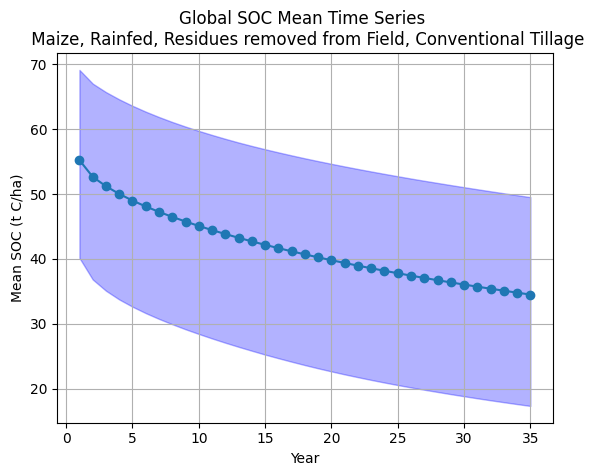
\includegraphics[width=0.85\textwidth]{SOC_LEAF_Example_25_0.png}
\caption{Example global SOC factor map (\si{\tonne\,C\per\hectare}) for a single crop and
management scenario, generated by the \texttt{sbtn\_leaf} pipeline. Cool-to-warm shading
spans low to high SOC stocks; colour limits use distribution-based cutoffs to suppress
extreme outliers.}
\label{fig:soc-maps}
\end{figure}

\begin{figure}[t]
\centering
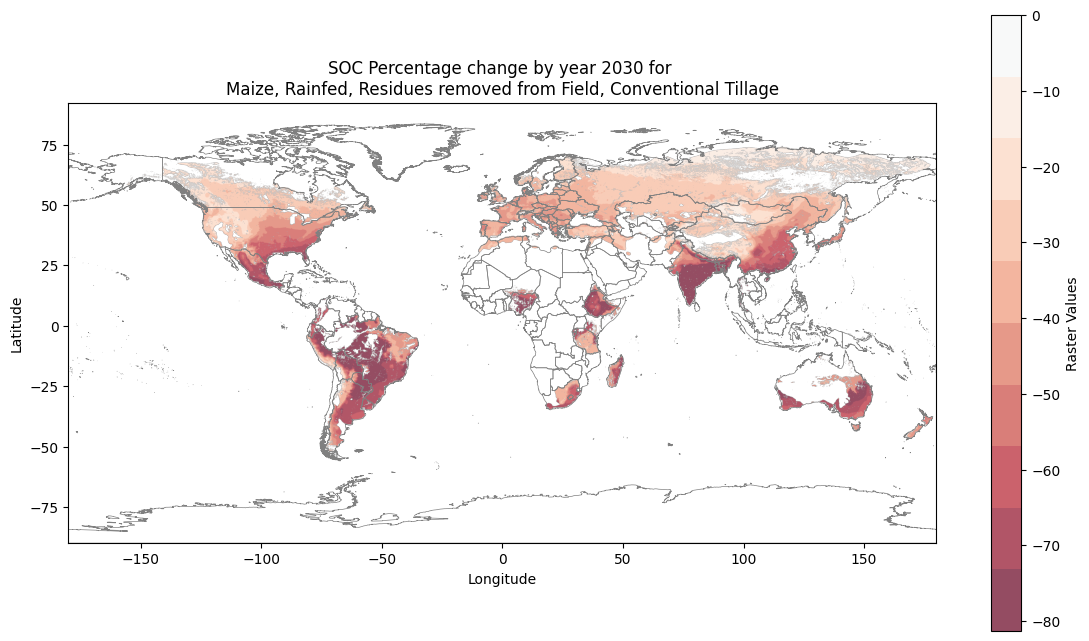
\includegraphics[width=0.78\textwidth]{SOC_LEAF_Example_31_2.png}
\caption{Projected SOC trajectory over the simulation horizon for a representative
maize scenario, showing the modelled change in soil carbon as land use is held constant
to 2030.}
\label{fig:soc-time}
\end{figure}

\subsection{Effect of land-management practices on SOC}
Because the same baseline is run under multiple management combinations, the factors
isolate the marginal effect of a practice change. Comparing conventional with reduced
tillage for rainfed barley with residues retained, across the 4{,}599 ecoregions where
both scenarios are defined, mean projected SOC rises from \SI{31.4}{} to
\SI{33.0}{\tonne\,C\per\hectare}---a gain of about \SI{1.6}{\tonne\,C\per\hectare}, or
\(\approx\)5\%. The benefit varies spatially with soil texture and climate, reflecting
the sand- and SOC-dependent tillage factor adapted from \citet{hyun2024}. These
practice-resolved differences are the quantity most directly useful for target setting,
since they estimate how far a management shift moves a landscape toward safe conditions.

\subsection{Global soil-erosion factors}
Baseline soil-erosion factors, aggregated to ecoregions across all land-use classes,
average \SI{48.8}{\tonne\per\hectare\per\year} with a much lower median of
\SI{15.3}{\tonne\per\hectare\per\year}, reflecting a strongly right-skewed distribution
in which steep, erosive, high-rainfall landscapes dominate the mean. Conservation
practices reduce these rates multiplicatively: reduced tillage alone scales erosion by
$C_{\text{till}}=0.35$ and no-till by $0.25$, with further reductions from residue
retention and cover crops, so that the modelled erosion factor under a full conservation
package can fall to a small fraction of the baseline.

\subsection{Terrestrial-acidification factors}
The acidification factors differ markedly among gases and biogeographic realms. Ecoregion
mean factors are \SI{0.24}{}, \SI{0.80}{}, and \SI{1.33}{\kilogram} \ce{SO2}-eq per
\si{\kilogram} for \ce{NO_x}, \ce{SO2}, and \ce{NH3} respectively, with maxima exceeding
\SI{25}{} for \ce{NH3} in the most sensitive soils. For \ce{NO_x}, realm-mean factors
range from \SI{0.018}{} in Oceania and \SI{0.061}{} in Australasia to \SI{0.31}{} in the
Nearctic and \SI{0.48}{} in the Palearctic (Figure~\ref{fig:acid}), spanning more than an
order of magnitude. This variability underscores why spatially explicit factors matter:
a single global value would misrepresent acidification impacts by realm by a large
factor.

\begin{figure}[t]
\centering
% Placeholder: regenerate from paper/Paper_Graphs_Figures.ipynb ("Boxplot showing
% differences per realm"). See manuscript README.
\fbox{\parbox[c][0.30\textheight][c]{0.8\textwidth}{\centering\itshape
Figure placeholder --- terrestrial-acidification factor (\ce{SO2}-eq) by biogeographic
realm, shown as boxplots per realm for \ce{NO_x}, \ce{SO2}, and \ce{NH3}. Regenerate by
running \texttt{paper/Paper\_Graphs\_Figures.ipynb} (section ``Terrestrial
Acidification'').}}
\caption{Distribution of terrestrial-acidification factors across ecoregions, grouped by
biogeographic realm. Realm means for \ce{NO_x} range from \(\approx\)0.02 (Oceania) to
\(\approx\)0.48 (Palearctic) \si{\kilogram} \ce{SO2}-eq per \si{\kilogram} emitted.}
\label{fig:acid}
\end{figure}

\subsection{Validation of yield inputs}
Because residue inputs depend on yields, the gap-filling procedure
(Section~\ref{sec:soc}) was examined against its FAOSTAT and SPAM sources. Raw SPAM
yields contain implausibly high values in a small number of pixels; restricting the
comparison to the 5th--95th percentile range removes these artifacts and brings the
spatial yield distribution into agreement with national statistics. This filtering, and
the hierarchical fallback that prefers spatially disaggregated SPAM data and only resorts
to ecoregion, biome, and nearest-neighbour estimates where necessary, limit the
propagation of yield outliers into the SOC factors.

\section{Discussion}
\label{sec:discussion}

\paragraph{Significance.} LEAFs provide, to our knowledge, the first openly licensed,
globally complete, ecoregion-resolved set of default factors spanning three soil-quality
indicators and built specifically for science-based land target setting. By combining a
process model (RothC) for SOC with empirical models for erosion (RUSLE) and acidification
(fate--sensitivity factors), and by resolving management scenarios explicitly, the
dataset lets companies estimate both their current position relative to ecoregional
thresholds and the expected effect of changing practices---all without primary field
data, while retaining the option to substitute such data through the same reproducible
pipeline.

\paragraph{Relation to prior work.} The SOC component extends the global RothC
implementation of \citet{morais2019} and \citet{teixeira2021} with practice-resolved
scenarios, an updated conservation-tillage factor \citep{hyun2024}, and a transparent,
tested software package. The erosion and acidification components adopt established
global datasets \citep{borrelli2017,panagos2015,roy2014} and harmonize them onto the same
spatial framework, which is itself a contribution: a single, consistent grid and
aggregation scheme makes the three indicators directly comparable across geographies.

\paragraph{Limitations.} Several simplifications should be borne in mind. SOC factors use
a 15~cm effective sampling depth as a proxy dictated by the 0--30~cm SoilGrids product,
and a single 2016 baseline projected forward under constant land use; companies with
land-use history can instead reconstruct current SOC and project from there using the
documented procedure. The DPM/RPM partition is held at standard literature values rather
than calibrated locally. Soil-erosion factors inherit the 25~km resolution and
assumptions of the GloSEM base layers and adopt the common $P=1$ simplification, which
omits support practices such as terracing and contouring. Yield gap-filling, while
guarded by percentile filtering, introduces uncertainty in data-sparse regions.
Acidification factors are inherited from a published method and are not re-modelled.
Finally, ecoregion and especially country averages mask within-unit heterogeneity;
native-resolution rasters should be preferred where the geometry of a sourcing landscape
is known.

\paragraph{Future work.} Planned extensions include reporting and refining the effective
UHTH resolution, adding farmyard-manure inputs and additional commodities to the SOC
scenarios, propagating input uncertainty into factor uncertainty, and publishing a
permanent archive of the native-resolution rasters alongside the summary tables.

\section{Data and Code Availability}
\label{sec:availability}
The complete source code (the \texttt{sbtn\_leaf} package), theoretical documentation,
executable example notebooks, and precomputed factor tables for SOC, soil erosion, and
terrestrial acidification are available in the project repository under a CC0~1.0
Universal (public-domain) dedication. Summary factors are provided as CSV tables and
GeoPackages for ecoregion, country, and subcountry units; native-resolution rasters are
distributed separately because of their size. The example notebooks reproduce the full
workflow from harmonized inputs to exported factors, enabling users to regenerate the
published factors or to derive customized factors from primary data.

\section*{Acknowledgments}
This work was developed by WWF in support of the Science Based Targets Network Land
methodology. We thank the authors of the underlying datasets and models---SoilGrids,
GloSEM, NASA GPM and GLDAS, FAOSTAT, SPAM, and the RothC, RUSLE, and acidification
modelling communities---whose openly available work makes these factors possible.

\bibliographystyle{plainnat}
\bibliography{references}

\end{document}
